\documentclass[a4paper,11pt]{report}
\author{Jiannan Guo}
%\usepackage[margin=1in]{geometry} %Prithvi

\usepackage[T1]{fontenc}

\usepackage{courier}
% defines\textmu etc
\usepackage{textcomp} 

\usepackage{lmodern}

\usepackage[latin1]{inputenc}

\usepackage[english]{babel}
%\usepackage{nada-ex}

% graphics and images
\usepackage{graphicx}
\graphicspath{ {./images/} }

% listings
\usepackage{listings}
\lstset{basicstyle=\footnotesize\ttfamily,breaklines=true}

% makes color citations
\usepackage[hyperfootnotes=false]{hyperref}
\hypersetup{
  colorlinks=True,
  citecolor=blue,
  linkcolor=black,
  urlcolor=blue}

% Appendix package
\usepackage[toc,page]{appendix}

% Tables multirow entries
\usepackage{multirow}

% Acronyms package - Prithvi
\usepackage[nonumberlist,acronym,toc,shortcuts,nomain]{glossaries}
\robustify{\gls}% Make \gls not fragile
%\loadglsentries[main]{acronyms}
\makeglossaries
% cmd to the folder and "makeglossaries acronyms"

% Header customization
\usepackage{fancyhdr}
\pagestyle{fancy}
%\renewcommand{\headrulewidth}{0pt}
\fancyhf{}
\fancyhead[l]{\slshape\nouppercase{\leftmark}}
\fancyhead[r]{\thepage}

%To point to the top of image/table on clicking a reference - Prithvi
\usepackage[all]{hypcap}
	
%For title page date - Prithvi
\usepackage[long,nodayofweek]{datetime}
\newdate{date}{15}{09}{2014}

% Biblatex - Prithvi
%Citation engine
%\usepackage[backend=biber,citestyle=ieee,urldate=long,doi=false,isbn=false]{biblatex}

%Source for citation
%\addbibresource{test-master.bib,rfc.bib}

%Use 'Retrieved on' for webpages cited
%\DefineBibliographyStrings{english}{%
%urlseen = {Retrieved on},
%}

%Include url and url date only for misc entries
%\AtEveryBibitem{\ifentrytype{misc}{}{
%    \clearfield{url}
%    \clearfield{urldate}
%  }
%}

%%%%%%%%%%%%%%%%%%%%%%%%%%%%%%%%%%%%%%%%%%%%%%%%%%%%%%%%%%%%%%%%%%%%%%%%%%%
%TODO fix template - in progress (Prithvi template)
\begin{document}

% Title page
\begin{titlepage}
\thispagestyle{empty}

\begin{center}
%  \includegraphics[height=6cm]{kth_cmyk_info_comm_tech}\\
  \vspace{0.5cm}
  \Large{\sc KTH Royal Institute of Technology}\\
  \vspace{3cm}

  \vspace{0.5cm}
  \Large{Highly Available and Robust Network Services in Under-served Areas}\\
  %\vspace{0.5cm}
  \vspace{2cm}  
  \large{\sc Jiannan Guo}\\
  \vspace{3cm}
  Master's thesis\\
  \vspace{0.5cm}
  \begin{tabular}{ll} 
    %TODO tranform o to swedish o
    Supervisor: & Prof. Bj\"{o}rn Pehrson, KTH\\		
	Examiner:  & Prof. Markus Hidell, KTH\\ 
  \end{tabular}
  \vspace{1cm}
  \\Stockholm, \displaydate{date}\\
\end{center} 

\end{titlepage}

% Prefix (abstract, contents etc.)
\pagenumbering{roman}
\pagestyle{plain}
%\include{0.prefix}

% Main text
\cleardoublepage
\pagenumbering{arabic}
\pagestyle{fancy}

\part{Robust Network Infrastructure in Rural Areas of Tanzania}

\part{Highly Available Web Services}

\chapter{Introduction}

In this chapter, we introduce the motivation to build a highly available web service in rural area. We illustrate the result of observation and identify the key problems.

In chapter \ref{sync}, we start by formulating the problem into a multi-master system, and then investigate several available technologies that address this challenge. We examine them against our unique requirement and select one as our basis. We then propose and explain our approach on top of it.

In chapter \ref{benchmark}, we illustrate the idea of using ARM-based hardware to achieve low-power consumption web service. To study the capacity of hardware, we benchmark the performance of each components of web service on different platform. According to the result, we propose a cluster than can be easily scaled out to serve more users.

In chapter \ref{conclusion}, we draw our conclusion and shed light on future work.
\section{Background}
Affordable, yet stable web services are highly desired in rural area, as a mean to alleviate digital divide and improve life quality. When it comes to under-developed regions in Africa, requirements and conditions need to be carefully assessed and analyzed, for that challenges could be unique and dramatically different than metropolitan.

\section{E-learning for Open University of Tanzania} \label{out_intro}
%database-driven and static
Open University of Tanzania (OUT) \cite{out} is the first university of East Africa Region to provide open and distance learning programmes. To distribute course content through the whole country, Moodle has been chosen as underlying digital resource management platform. Moodle\cite{moodle} is an open-source industrial-level online learning platform and resource management system. As a typical data-driven web service, Moodle runs over an underlying database and assemble its webpages on-the-fly based on user requests. It is written in PHP and heavily tested against Apache, Nginx and MySQL. At present, the platform is running as a standalone web service in a central server and mainly serve static content such as PDF, Text and Slides. Although OUT has the vision to introduce multi-media materials to enhance education quality. OUT also establishes learning centers in major cities and towns all over the whole country and is ambitious to extend to a larger scale. An emerging obstacle is to provide services in remote areas with poor network connection and bandwidth.

\section{Problem Identification}
%Objectives to achieve in this projects.
%Goals
As part of the project, we investigated local conditions and needs within the scale of Serengeti Broadband Network, especially in areas with evident demands of services and lack of infrastructures. And we were able to identify following challenges:

\subsection{Power Outages}
%ellaborate this paragraph
Power grid in rural areas of Tanzania is so unreliable that UPS for critical device is almost a must. While people are gradually adapting to mobile platforms, such as smart phones and tablets, backbone infrastructures are also required to be more persistent. Equipments powered up by solar and battery are highly desired due to cost-efficiency. Although power consumption need to be optimized in this circumstance in order to prolong battery life and improve reliability.

\subsection{Poor network quality and frequent failure}
Although local network is operated by ICT4RD project and can be fairly reliable, uplink is still depending on national-wide ISP and is somewhat unpredictable according to our observation. Network failure could occur anytime and can last for random period (several minutes to several days). Those web services that depend on a central server are apparently not accessible during the failure. On the other hand, the uplink can be very narrow due to poor infrastructure and limited budget. It could be difficult to squeeze multimedia services into such bandwidth.

To better illustrate this problem, suppose a typical setting in Figure \ref{rural_lan}. Major backbone components in this LAN are interconnected through fiber-optical lines, and network is distributed to users through WiFi or Ethernet. The LAN is linked to the Internet through ISP distribution link and central server resides on the otherside of the Internet.

\begin{figure}[htbp]
\centering
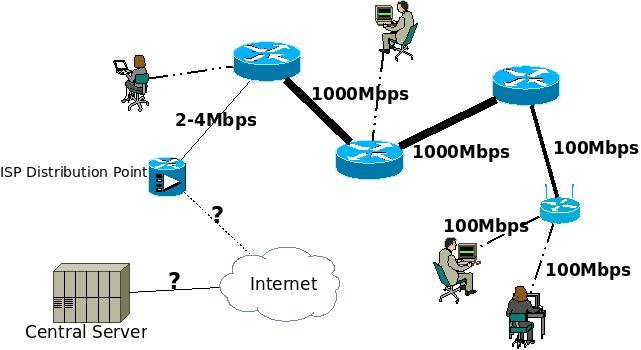
\includegraphics[width=0.8\textwidth]{../images/brief_diagram_of_sbn_network.jpeg}
\caption{A Typical Setting of Rural Local Access Network (LAN)}
\label{rural_lan}
\end{figure}

Due to limited budget and ISP capacity, the upper link is equipped with an average bandwidth of 2~4Mbps which is shared among all users in LAN. While a minimum bandwidth of 1.5Mbps is recommended for video streaming, it is difficult for users to get decent service from central server.
To worsen the situation, the upper link is somewhat unpreditable, which leads to the isolation of LAN, as shown in \ref{uplink_break}.

\begin{figure}[htbp]
\centering
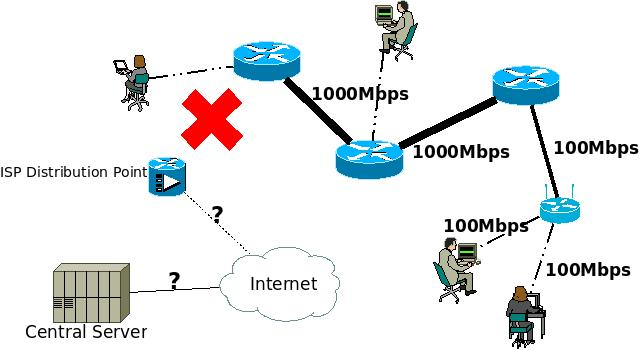
\includegraphics[width=0.8\textwidth]{../images/brief_diagram_of_sbn_network_upper_broken.jpeg}
\caption{Uplink Failure leads to the isolation of LAN}
\label{uplink_break}
\end{figure}

On the other hand, components in the LAN can also break down which leads to network separation, see Figure \ref{nata_break}. In the first case, multi-media content can hardly reach end users. And in other two cases, users cannot get service at all.

\begin{figure}[htbp]
\centering
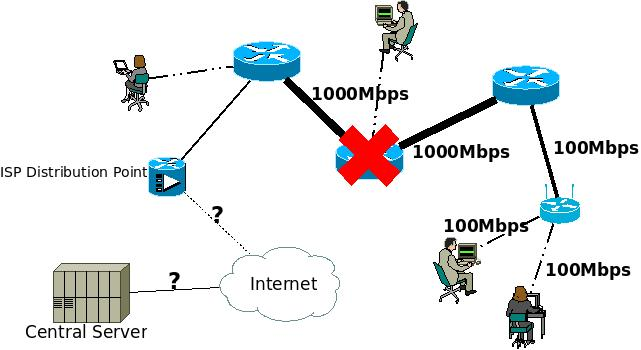
\includegraphics[width=0.8\textwidth]{../images/brief_diagram_of_sbn_network_nata_broken.jpeg}
\caption{Network Separation due to Component Failure}
\label{nata_break}
\end{figure}

\subsection{Limited budget}
Cost is an essential factor during rural ICT development. Given relatively smaller user base and weaker demand, equipments need to be chosen wisely. Although future maintainence and development also need to be considered.
\chapter{Adapt to Frequent Network Failure and Limited Bandwidth}\label{sync}
In this chapter, problems are further decomposed and analyzed. To prevent reinventing-the-wheel, a variety of possible solutions are proposed and investigated, whereas focus has been put into our unique requirements.

%Most of techniques today focus on reducing response time and improving concurrency, rather than offline operation and network partitioning. Even though major companies optimize their server architecture for miliseconds of faster, web service in rural areas is still a question of existance.

%TODO Read-only and Read-write

%Overall goals are:
%\begin{itemize}
%\item To reduce user-perceived latency and bandwidth usage within the context of rural LAN with a narrow upper link.
%\item To serve up-to-date content.
%\item To achieve partition tolerance by continuing service when network failure occurs.
%\end{itemize}

\section{A closer look at the problem} \label{components}
As introduced in section \ref{out_intro}, Moodle is deployed as underlying course management system for OUT E-learning platform. Moodle is an open sourse project written in PHP and well-documented\cite{aosamoodle}\cite{moodledoc}. Similiar to other web applications, it can be deployed in a typical LAMP or LNMP stack. In this chapter, we mainly focus on possible solutions for two problems stated previously, and leave the choice of actual server to chapter \ref{benchmark}

%Moodle components
Moodle is a typical database-driven web application where all the pages are generated on-the-fly based on user request. The whole application is composed of three main components: 
\begin{itemize}
\item PHP source code, typically in \texttt{/var/www/moodle/}
\item A database to store data or metadata including site configuration, student information, course details, events, etc. There exist volatile tables in Moodle database which store sessions and temparory information.
\item A directory to store materials and resources, as well as cache and temparory files. Typically it is named as \texttt{moodledata/}
\end{itemize}

%model of problem
The problem addressed previously can be simplified and modelised as following,
see Figure \ref{problem_model}. Each node in the model denotes a local
server/proxy and has a certain amount of users associated with it.

\begin{figure}[htbp]
\centering
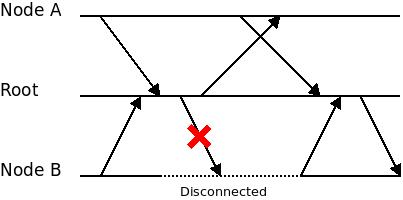
\includegraphics[width=0.6\textwidth]{../images/model_centralized.jpeg}
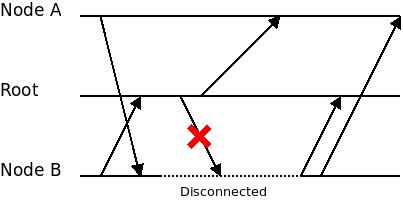
\includegraphics[width=0.6\textwidth]{../images/model_distributed.jpeg}
\caption{Web Delivery Model}
\label{problem_model}
\end{figure}

%What to store
As simple as the model might be, components in it could be vastly heterogenous if mapped to different techniques. Content stored in a node can either be web objects, SQL replies, codes or even entire databases. Communication in between can also be based on a variety of protocols.

%Interactive session
As an online learning platform, users do not only passivly accept information, but also interact with Moodle through forum, personal blogs and quiz. All the changes made by users must be stored and seen everywhere. Thus, the system should not be read-only under any circumstance.

%Dynamic content


%production and minimum affection
Moodle has been in service and adding new services should affect existing structure as less as possible. Also, steps of adapting changes should be properly designed to avoid crushing the service.

%communication overhead
To maintain consistency and serve up-to-date content, a reasonable amount of
communication overhead is necessary and is normally positive proportional to the
extent of consistency. Although, due to the presumption of poor network
connection and narrow bandwidth, different nodes in the system are preferably
decoupled and autonomous.

%Offline operation
The autonomy is also closely correlated to the ability of performing offline operation. Many distributed systems have the ability to detect and recover from network partitioning, although it normally leads to a compromise of consistensy and content freshness. When a user request a page, Moodle loads all previliges of the user, generate pages accordingly and log the session. This results in uncacheble content and interaction-must logins. It has been proven that consistency, high availability and partition tolerence are impossible to be achieved at same time\cite{brewer2000towards}\cite{gilbert2002brewer}, necessary trade-off has to be made according to the condition and needs.

While the majority of web caching and content distribution techniques aim at better performance and delivery efficiency, we prioritize the ability of performing basic functionalities during network failure. We tolerate a relatively loose consistency while ensuring eventual convergence.

%Affordability
Lastly, to realize affordability, we mainly focus on open source techniques and free ware. Thankfully, many successful projects and tools have been made open source and publicly available. In the following sections of this chapter, we evaluate a variety of techniques against the criteria stated above and propose our solution based upon the conclusion. Several of potential solution are also tried out.


\section{Push Web Service to Edge}
\subsection{Content Delivery Network}
Content Delivery Network overlaps with Web Cache Proxy at the concept of pushing web content to users. A Content Delivery Network is a collaborative set of surrogate servers spanning the network, where web contents are mirrored\cite{pathan2008content}. Users will perceive a smaller latency while fetching content from a nearby CDN surrogate server rather than original web server. The essence of CDN is illustrated in Figure \ref{cdn}.

\begin{figure}[htbp]
\centering
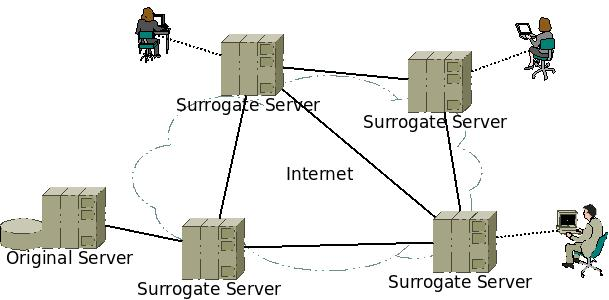
\includegraphics[width=0.8\textwidth]{cdn.jpeg}
\caption{Content Distribution Network}
\label{cdn}
\end{figure}

Since more and more web services are evolving to provide dynamic content, CDN also takes advantages of cachebility hints when dealing with dynamic contents\cite{dilley2002globally}. 

%TODO open source CDN project

\subsection{Simple Web Caching}
An intuitive and common solution for the problem of limited bandwidth is to cache popular web content locally, as illustrated in Figure \ref{with_cache}.
A client-side web cache proxy is typically deployed in user local network, requesting web servers on behalf of users, and cache web objects for further references. Web caching has been proven to be an effective approach to reduce bandwidth usage, user-perceived latency and loads on original server\cite{davison2001web}.

\begin{figure}[h]
\centering
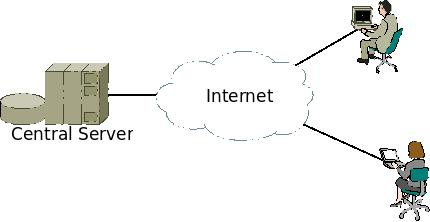
\includegraphics[width=0.6\textwidth]{../images/without_caching.jpeg}
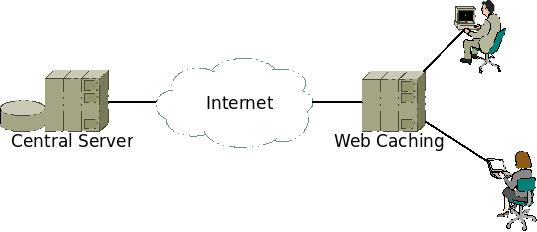
\includegraphics[width=0.6\textwidth]{../images/with_caching.jpeg}
\caption{Serve users without and with a Gateway Cache}
\label{with_cache}
\end{figure}

Web cache is greatly advantageous in our scenario that it does not require modification on web application, except that some TCP optimizations could be done between web cache proxy and web server frontend. Web cache proxy can continue serving requests with offline mode enabled, which also meets our requirements. The traffic between cache proxy and authentic server is standard HTTP request and response. The overhead and frequency of communication mainly depends on cache hit / cache miss ratio, expiration time and cache directory size.

Although, this solution encounters two major constraints in our case:
\begin{itemize}
\item Moodle pages are generated on-the-fly based on user information. Web cache cannot operate on its own during network failures, except for serving previously requested pages.
\item Users are required to log in to browse. Thus, user-server interactions are always necessary, which also contradict with our purposes.
\end{itemize}

%One important feature of all web cache proxies is replacement strategy which invalidate caches and maintain freshness. A comprehensive survey of existing replacement strategy is presented in \cite{podlipnig2003survey}. However

\subsection{Page generation on Edge Server}
To address the issue of dynamic content generation and client-server interaction, an intuitive and brute-force solution is to generate user-specific page at the edge. A comprehensive study of edge servers can be found in \cite{pathan2008content}. Four strategies are presented: (a) edge computing (b) content-aware caching (CAC) (c) content-blind caching (CBC) (d) data replication.
%TODO replication figure
In each of the strategy, the edge server attempts to reply user request on the behalf of original server with the information that is locally available. Edge computing still heavily relies on central database, hence out of our consideration. While CAC and CBC store partial database at the edge, data replication stores a complete copy of the database.

If the size and complexity of database permit, data replication is desired since it outperforms other strategies in both response speed and offline operation. Although, it adds another layer of complexity to perform transaction processing and maintain the consistency through mutliple distributed databases. Techniques to achieve a consistent distributed database system are presented in section \ref{database_sync}.

Application code rarely changes in our case and is always one-way synchronized from original server, thus consistency can be relatively easy to achieve by periodically utilizing tools like rsync\cite{tridgell1999efficient}.

%TODO file system

\section{Multi-Master Database Synchronization} \label{database_sync}
As addressed previously, consistency, availability and partitioned-network cannot be accomplished at the same time, according to CAP theorem\ref{brewer2000towards}. Necessary trade-off has to be made to adapt to particular circumstance. Based on objectives defined previously, we prioritize availability and partitioned-network, while allowing loose consistency, as long as eventual consistency is guaranteed\ref{vogels2009eventually}. Pessimistic replication always guarantees consistent content perceived by users, thus widely adopted in distributed database system to enhance availability and performance. Although optimistic replication permits diverged databases, which is more suitable in our case. An exhaustive survey on optimistic replication is presented in \ref{saito2005optimistic}.

Comprehensive theoretical researches have been made available although we find limited open source implementations that serve our purposes. We investigate several data replication technologies in this section based on following criteria:
\begin{itemize}
\item \textbf{Deployment over WAN}
Most of distributed database system assumes a LAN environment, where delay and bandwidth do not evidently affect exchange of data among servers. Although in our case, databases are deployed over WAN, which is highly unreliable and network latency is not neglectable.

\item \textbf{Serializibility}
To achieve eventual consistency, concurrent changes made at different edge servers need to be serialized. Hence, an order of operations is extracted based on relations among them.

\item \textbf{Conflict detection and reconsiliation}
\end{itemize}

 Several data replication technologies are investigated in this section in order to find a tool that requires minimum modifications to fit into our problem.

Distributed database system is widely adopted in server clusters and workstations, as a mean to enhance performance and redundancy. Although LAN is normally assumed by most of database replication technologies. 





%Database replication techniques has been intensively deployed over clusters and workstations for redundency and load balancing. A LAN is always assumed by most of database replication techniques, whereas database replicas across the WAN are desired to realize our goals. We prioritize availability by compromising on consistency, as long as the system can reach eventual consistency\cite{vogels2009eventually}. Offline operations on distributed databases often encounter simutaneous modification on the same entry, which result in conflict after reconnection. Techniques to detect and reconsile conflicts are studied and evaluated.
%TODO transaction process

\subsection{Database Cluster} \label{db_cluster}
%CouchDB
\textbf{CouchDB}\cite{couchdb} is an open source distributed database system developed in Apache. The most attractive feature of CouchDB is that it natively supports bi-directional synchronization among multiple database replicas and offline operations. When one replica is disconnected from the network, it retains autonomy and continues as a fully functional database from user point of view. Although, it fails to be our candidate since it is NoSQL database, whereas Moodle heavily relies on SQL calls and it will a significant task to modify Moodle to use NoSQL database.

%MySQL native replication
\textbf{MySQL Native Replication} is shipped with most of MySQL standard distributions that provide built-in functionalities to replicate databases. The synchronization is uni-directional that databases on master node are replicated to slave nodes. ALthough bidirectional synchronization can be achieved by creating loop in the topology. A simplest 2-nodes example can be found in Figure X. Node A and node B synchronize with each other by maintaining mutual dominance. The figure also shows a more complicated topology where three nodes comprise a loop. Although, the synchronization can be easily broken by conflict and the reconciliations always require human intervention.
To avoid insertion conflicts of auto-incremental keys, MySQL provides an option to increase incremental step. This feature is further discussed in section \ref{multi_master}

\begin{figure}[htbp]
\centering
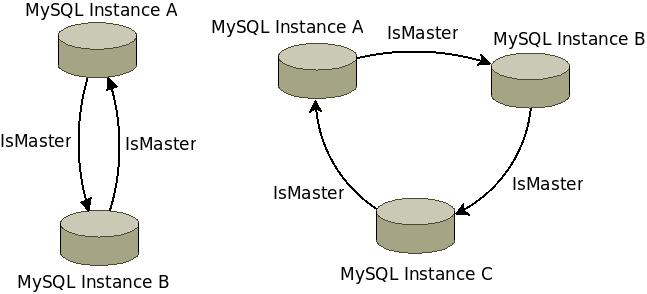
\includegraphics[width=0.7\textwidth]{mysql_repl.jpeg}
\caption{MySQL Replication}
\label{mysql_repl}
\end{figure}

%MySQL cluster
\textbf{MySQL Cluster}\cite{mysqlcluster} is an open source distributed database system based on MySQL. It supports database sharding and duplicating. A typical use case of MySQL Cluster is shown in Figure \ref{mysql_cluster}. Although, redundent copy of database can only be accessed with the presence of management master, and cannot be updated during network failures. Furthermore, database nodes are closely coupled with the assumption of LAN (low latency and high bandwidth).

\begin{figure}[htbp]
\centering
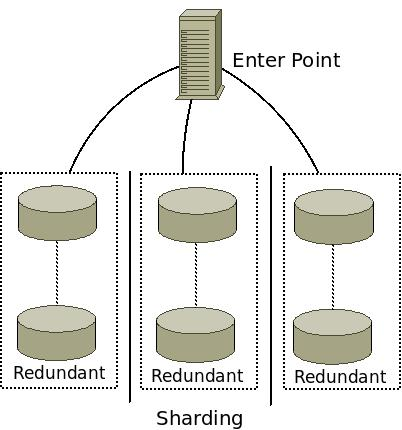
\includegraphics[width=0.4\textwidth]{mysql_cluster.jpeg}
\caption{MySQL Cluster}
\label{mysql_cluster}
\end{figure}

\subsection{Middleware-based Repliation System}
Several studies also proposed the approaches to solve database synchronization at middleware-level\cite{cecchetc}\cite{amza2003conflict}\cite{plattner2004ganymed}. C-JDBC \cite{cecchetc} is an Java implementation of RAIDb\cite{cecchet2005raidb}, aiming at a framework to manage heterogenous databases. With built-in functionality of scheduling transaction processes, C-JDBC is perceived by users as a single virtual database. Although, the system is still centrally managed and could not handle partitioned network. Ganymed middleware system\cite{plattner2004ganymed}, inspired by C-JDBC, achieves consistency by serializing update/write requests at master and propogating changes to replicas in a lazy fashion. Users see a consistent data state (snapshot isolation), even though stale might it be. The limitation of these two middleware is also clear, that no write can be served during network failures.


\subsection{Multi-Master Sycnhronization System} 
Similiar to MySQL Cluster Multi-Master setup, we found three state-of-the-art open source tools to the similiar end.
\begin{itemize}
\item \textbf{Galera}\cite{galera} is an open source synchronous database replication software developed to scale web application and provision high availability. It achieves consistency by optimistic locks and group communication. Galera is quorum-based and handles network partitioning by sacrificing the minority. Hence, Galera lacks the essencial features that we are seeking for and is out of consideration.
\item \textbf{Tungsten}\cite{tungsten} replicates database asynchronously and allows loose consistency. Transactions are commited locally, and then propogated across all other nodes. Tungsten features offline operation and automatical recovery although it leave the responsibility of conflict avoidance completely to the application. Conflicts may disturbe replication and hard to trace.
\item \textbf{SymmetricDS}\cite{symmetricds} is another open source asynchronous database replication management tool. It has several built-in rules to detect and reconsile conflicts. It can be configured flexibly to meet different needs, for example, have different courses store in different sites. Also, one appealing feature is that SymmetricDS support file synchronization as well. Figure \ref{symmetricds} birefly illustrates how SymmetricDS works and more details in terms of conflicts detection and reconsiliation are discussed in section \ref{multi_master}
\end{itemize}

\begin{figure}[htbp]
\centering
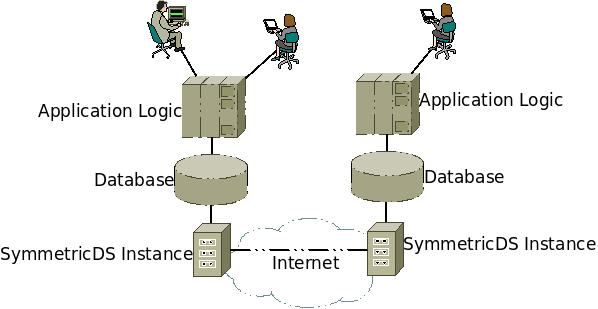
\includegraphics[width=0.8\textwidth]{symmetricds.jpeg}
\caption{SymmetricDS}
\label{symmetricds}
\end{figure}

We can conclude from above comparison that SymmetricDS is closest to our critaria and can be properly extended to meet our requirements. In the following section, we explore SymmetricDS in details and propose an approach to extend it.

\subsection{Conflicts Avoidance and Reconciliation} \label{multi_master}
Before we start illustrating our approaches for conflict detection and resolution, several reasonable application-specific assumptions need to be made:
\begin{itemize}
\item No user will attempt to login into two different server simutaneously, thus the content belong to this user will not be modified at two different sites.
\item Administration-related content is always synchronized through top-down approach, that is, user creation, deletion and modification are always synchronized in one-way.
\item No local user will be able to reply to a post that is not propogated to this edge server yet.
\item Volatile entries are not synchronized, such as cache and session.
\item Deletion wins. And events that causally follow the deletion also get deleted. If users reply to a post on a remote server whereas the post gets deleted on central server, all replies will get deleted once converged.
\end{itemize}

As introduced in section \ref{db_cluster}, insertion conflicts of primary keys can be avoided by setting different incremental steps, as long as the primary key is auto-incremented integer, see Table \ref{mysql_key_inc}.

\begin{table}[htbp]
\centering
\begin{tabular}{c|c|c|c}
Primary Key & Node A & Node B & Node C\\
\hline
1 & inseted by A & & \\
2 & & inserted by B & \\
3 & & & inserted by C \\
4 & inserted by A & & \\
5 & & inserted by B & \\
\end{tabular}
\caption{MySQL instances with different auto-incremental steps}
\label{mysql_key_inc}
\end{table}


Thankfully, all Moodle database tables are designed to use auto-incremental keys as primary key. By configuring incremental step and SymmetricDS, we are able to achieve a naive mutually consistent system. Configuring SymmetricDS is nontrivial and requires constant observation. Appendix A describes a work flow of configuring SymmetricDS.

Although, there are several major drawbacks of this design:
\begin{itemize}
\item It is not scalable. The incremental step limits the max number of servers in the system.
\item It is blind to application. It does not check logical correctness of modification according to application, e.g. replies to a previously deleted thread can still be inserted into database.
\end{itemize}

To attack these problems, we examine the way SymmetricDS handles conflicts and propose an extension that is more flexible and tunable. SymmetricDS applies the concept of CVS (Concurrent Versions System) to detect conflicts at a granularity of table entry level. When a node propogates a change on one table entry, it sends the before-state of that entry along with the change. Upon receipt, remote node compares the current state of this entry and the history. If they differ, a conflict is detected. Even though conflict resolution is highly application-specific, SymmetricDS provides limited rules to resolve known types of conflicts.

A SymmetricDS node can be configured to either actively pull from other nodes, or passively waiting for changes being pushed. While optimistic replications normally assume a negotiation phase while attempting a resolution, push and pull in SymmetricDS are independent from each other. Thus, conflicts resolution can be sometime confusing. For example, suppose a scenario in Figure \ref{sym_confuse}. Slave node is configured to push data to master while pulling changes from it. Since two operations are independent from each other, two replies to the same post are replaced by each other at two nodes, whereas the intention is to simply stack them.

\begin{figure}[htbp]
\centering
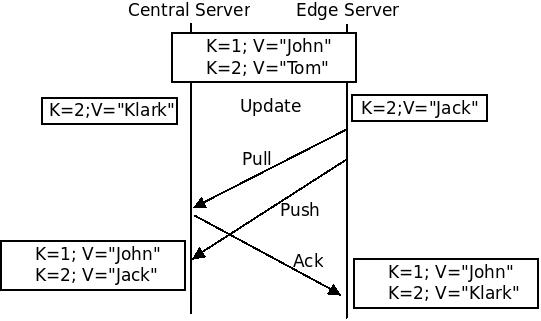
\includegraphics[width=0.8\textwidth]{sym_confuse.jpeg}
\caption{Misbahavior of SymmetricDS}
\label{sym_confuse}
\end{figure}

To attain serializibility, several repliation systems applies a centralized algorithm that serialize all changes at master node and then propogate to slaves. Although, it often requires a closely connected system and can suffer from latency and disconnection. Inspired by Git and Operational Transformation \cite{ellis1989concurrency}, we propose a distributed work flow in Figure X where conflicts are resolved at edge server, similiar to the mechanism used in Dropbox\cite{dropbox}. Edge node always pull the master first before commiting any changes. 
%TODO conflicts resolution work flow figure


\chapter{Low Power, yet Powerful}\label{benchmark}
The ARM-based processors have received great attention for its characteristic of low power consumption and energy efficiency, especially in smart phone and portable device industry, where power consumption is one the most critical specifications. Furthermore, there is trend in server industry to shift to ARM-based architecture in order to cut off the bill of electricity. ARM is also ambitious in this area and about to publicize processors capable of virtualization. When it comes to rural development, power shortage has been forcing researchers and engineers to seek for alternative power sources. Lower power consumption of the equipments implies a bigger potential of surviving severe environment.
Currently, we are exploring the possibilities of two platforms, namely Raspberry Pi and Odroid. The specifications of these two platform can be found in Table X
%TODO specification table
In the following sections, we benchmark a variety of attributes of Odroid and Raspberry Pi. The objective is to clarify the capacity of these two platforms and an optimum form to run the web service. We test every component of a complete Moodle installation to identify the bottleneck of the application. Based on the results, we propose the optimum cluster solution that can be easily scaled out to serve more users.

\section{Processor and Bandwidth Latency}


\section{Benchmark of Web Components}
To test components of a complete Moodle installation, we design a expirement in Figure X. Each part is respectively substituted with either Odroid or Raspberry Pi, and remaining parts are running on a high-end machine which is much more powerful than these two platforms, in order to put enough siege on the testing target. Furthermore, simulated requests are generated from high-end machine as well.

\section{Web Frontend}
Most of the websites today are powered by Apache due to its long history and abundant extensions. Although Apache relies on a processed-based manner to handle new connection, which has limited the scalability and concurrency. Nginx is an event-based reverse proxy that handles request asynchronizily. It addresses C10K problem from the beginning and focus on scalability.
To determine which server runs better on a resource constraint platform, we benchmark Nginx and Apache on both platform to evaluate the throughput, level of concurrency and response delay. We use siege to generate workload and compare the performance of web server with two different type of object: small text file and large JPG file.
We siege the server in following setting:
%TODO topology

\begin{figure}[h]
\centering
\begin{subfigure}{0.45\textwidth}
\centering
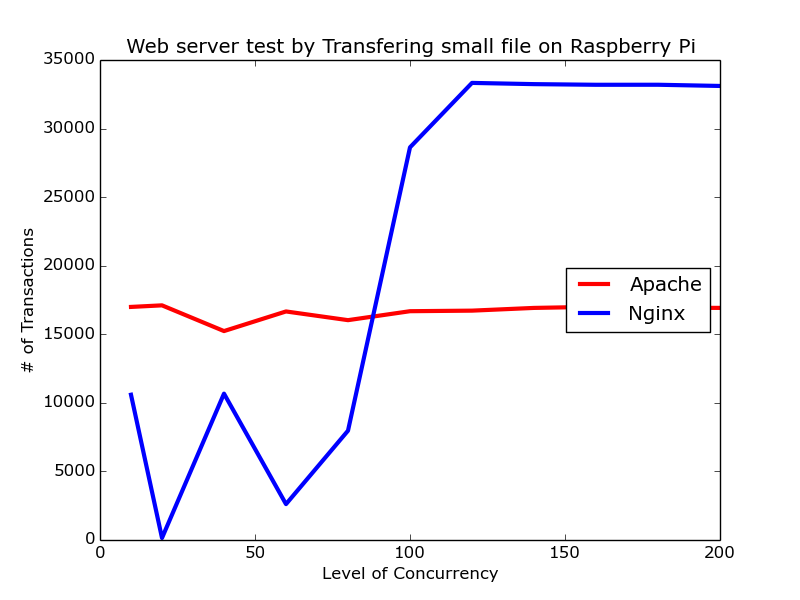
\includegraphics[width=\textwidth]{rpi_small_text.png}
\caption{Raspberry Pi (small text file)}
\end{subfigure}
\begin{subfigure}{0.45\textwidth}
\centering
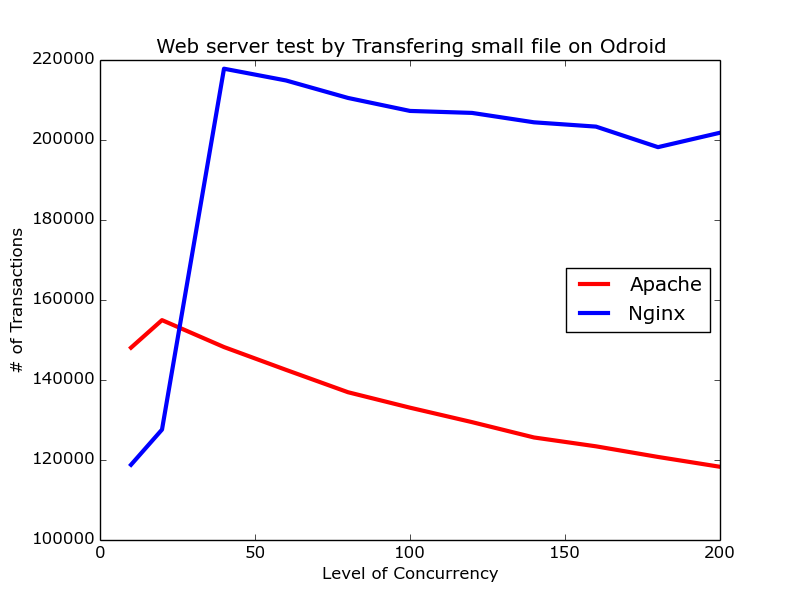
\includegraphics[width=\textwidth]{odroid_small_text.png}
\caption{Odroid (small text file)}
\end{subfigure}

\begin{subfigure}{0.45\textwidth}
\centering
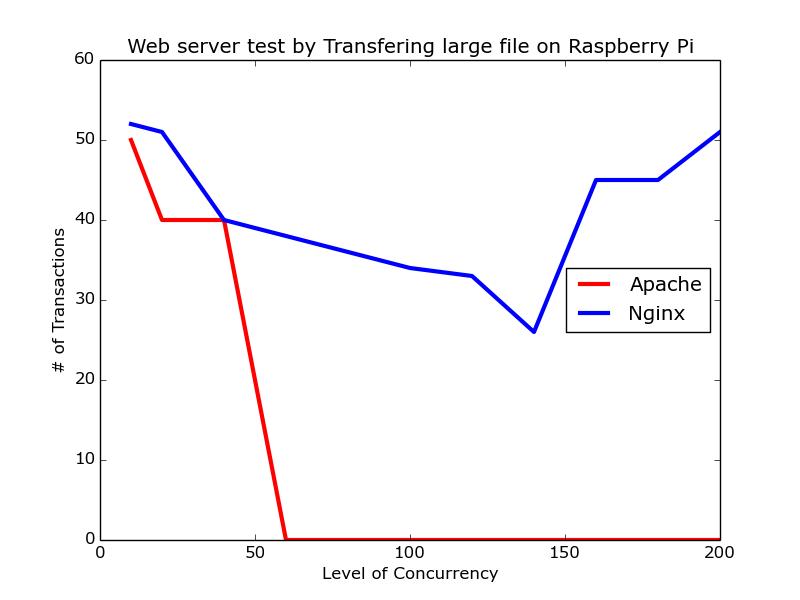
\includegraphics[width=\textwidth]{rpi_big_jpg.png}
\caption{Raspberry Pi (big jpg file)}
\end{subfigure}
\begin{subfigure}{0.45\textwidth}
\centering
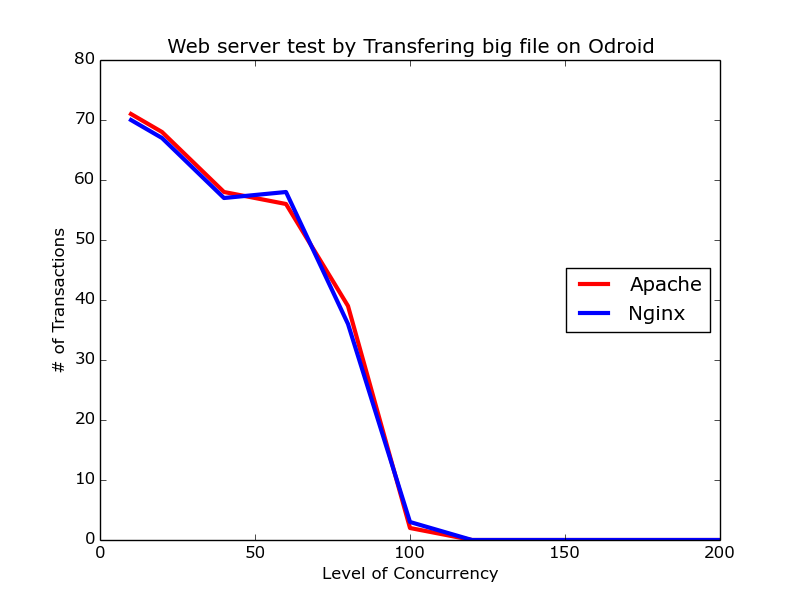
\includegraphics[width=\textwidth]{odroid_big_jpg.png}
\caption{Odroid (big jpg file)}
\end{subfigure}

\caption{A Benchmark of static file request on both platforms}
\label{static}
\end{figure}
%TODO figure
As shown if Figure \ref{static}, Nginx and Apache achieve comparable performance under a low level of concurrency, although Nginx outperforms Apache notebly when concurrency level increases. To be noticed, both web servers perform indistinguishably while serving large file. We observe fully occupied CPU in this specific test, which is due to intensive OS kernel processing of socket manipulation and packet tranfer. The impact of web server on the CPU is neglectable in this circumstance. Thus, expirement result in Figure \ref{static}(d) does not denote same performance of web servers.

\section{PHP Processing}
As a large PHP application, Moodle requires significant computational resources for PHP processing. Thus, a testbed is formed to benchmark PHP processing capacity of two platforms, see Figure X
%TODO PHP benchmark testbed
The inputs are two different PHP scripts:
\begin{itemize}
\item a php script simply echoes \texttt{Hello, world!}
\item Moodle index page which requires heavy php processing.
\end{itemize}

\begin{figure}[h]
\centering
\begin{subfigure}{0.45\textwidth}
\centering
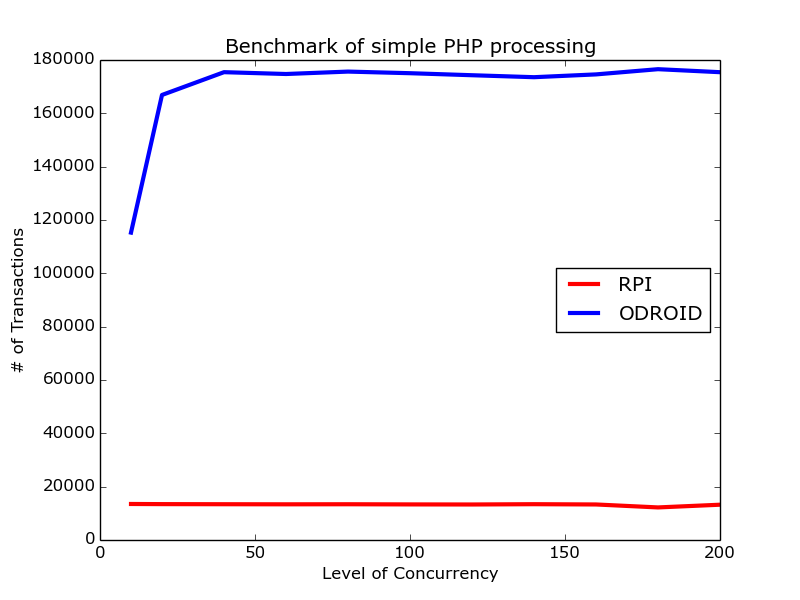
\includegraphics[width=\textwidth]{simple_php.png}
\caption{$\sum trans$}
\end{subfigure}
\begin{subfigure}{0.45\textwidth}
\centering
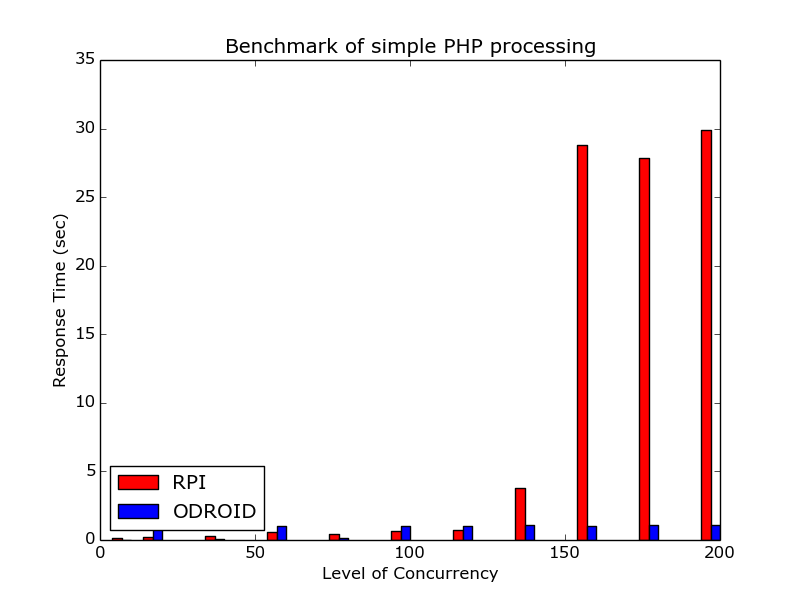
\includegraphics[width=\textwidth]{simple_php_max_res.png}
\caption{Longest Response Time}
\end{subfigure}
\caption{A Benchmark of simple PHP processing on both platforms}
\label{simple_php}
\end{figure}

Figure \ref{simple_php}(a) shows that Odroid can handle much more PHP request than Raspberry Pi. Overall response time is shorter for Odroid. Although, half of the CPU usage is taken by OS kernel during these two test and the difference satisfactorily convincing. The gap between two platforms is more evident when tested with heavier PHP processing, as shown in Figure \ref{moodle_php_result}.\footnote{We observe a 6~7 seconds delay to process index page of Moodle on Raspberry Pi and it can barely tolerate the mildest siege. Thus, the test result of Raspberry Pi is left out in this test.}

\begin{figure}[h]
\centering
\begin{subfigure}{0.45\textwidth}
\centering
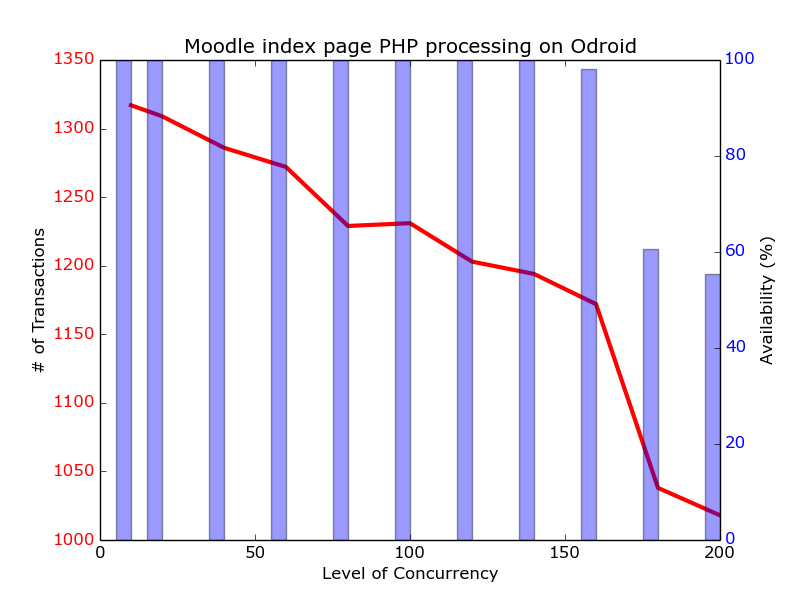
\includegraphics[width=\textwidth]{moodle_index.png}
\caption{$\sum trans$ \& Availability}
\end{subfigure}
\begin{subfigure}{0.45\textwidth}
\centering
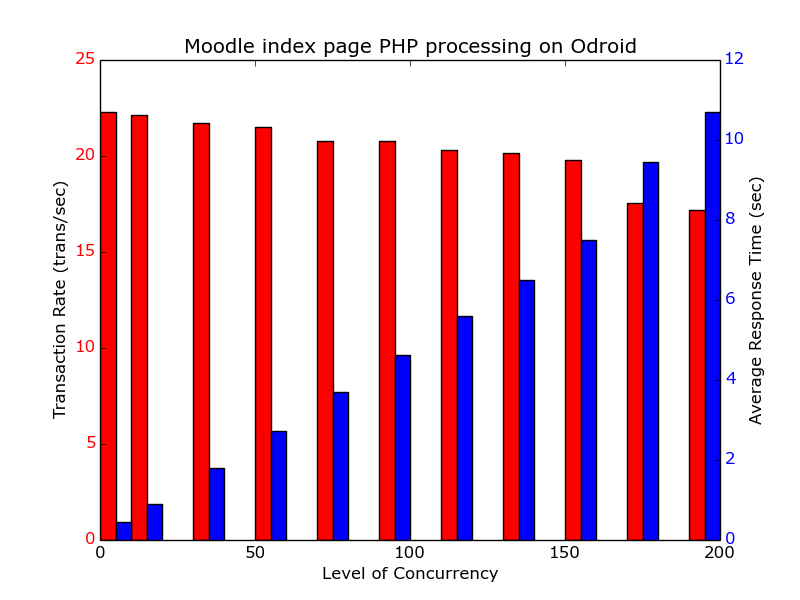
\includegraphics[width=\textwidth]{moodle_index_2.png}
\caption{$Rate_{trans}$ \& $T_{resp}$}
\end{subfigure}
\caption{Moodle index processing on Odroid}
\label{moodle_php_result}
\end{figure}

As shown in Figure\ref{moodle_php_result}(a), transaction rate and availability drops under 180 concurrent requests occur. The latency is beyond tolerable under 50 concurrent requests, according to a study of tolerable waiting time of website\ref{}. As the total transaction number in this test is significantly lower than the previous one in Figure \ref{simple_php}, we suspect that PHP processing power is the bottleneck in a moodle installation rather than database query and web frontend. Thus, we test the capacity of a standalone installation of Moodle, in which all components are in one box (Odroid), shown in Figure {}

Impact of changing web frontend does not evidently influence transaction rate, which implies that PHP processing capacity is the limiting factor in one Moodle installation.

\section{Database}
We apply the same method to test database although fail to exhaust the resource on Odroid before running out CPU and memory on our testbed high-end machine, hence we conclud that database query does not limit a Moodle installation before expanding PHP capacity.

\section{Scale Out to Eliminate Bottleneck}
We propose following cluster structure that can be easily scaled out coinciding the increase of users, see Figure \ref{}
%TODO cluster figure


\chapter{Conclusion and Future Work}\label{conclusion}
\section{Conclusion}
Starting from the user case, by applying the concept of divide-and-conquer, we are able to formulate the problem and identify the key challenges. Given the impossibility of achieving consistency and availability at the same time, we propose a multi-master system with reasonable assumptions and compromises. We surveyed a variety of existing technologies and investigate the potential to map them into our case. With extensions and proper configurations, SymmetricDS is tuned to serve our purpose. To achieve low-power consumption and affordability, we test the capacity and proposed a cluster which can be easily scaled out. We build Moodle web service on the cluster with integrated synchronization functionalities. We conclude that this prototype has the potential to serve in rural areas where highly available web services are desired and number of users is limited.
\section{Future Work}
At the beginning, the plan was to implement the system and test it in production environment. Although enormous effort has been put into exploring the possibilities of a variety of technologies. Also the overhead to adapt to local work culture unexpectedly disturbs original plan. Thus, the next step will be testing and debugging the system in a real production service. Also, the system can be generalized to serve other database-driven applications although proper configuration and modification are required. This potential should be further investigated.


\cleardoublepage
\phantomsection
\addcontentsline{toc}{chapter}{Bibliography}
\bibliography{master}
\bibliographystyle{IEEEtran}
%\printbibliography[title={Bibliography}]

%\include{appendix}

\end{document}
